\documentclass[aspectratio=169,11pt]{beamer}
\usetheme{Madrid}
\usecolortheme{seahorse}
\usefonttheme{professionalfonts}

\usepackage{amsmath,amssymb,bm}
\usepackage{booktabs}
\usepackage{array}
\usepackage{tikz}
\usetikzlibrary{positioning}
\usepackage{listings}
\usepackage{xcolor}
\usepackage{xeCJK}
\usepackage{fontspec}
\usepackage{hyperref}

\setmainfont{texgyreheros-regular.otf}[BoldFont=texgyreheros-bold.otf,ItalicFont=texgyreheros-italic.otf]
\setsansfont{texgyreheros-regular.otf}[BoldFont=texgyreheros-bold.otf,ItalicFont=texgyreheros-italic.otf]
\setmonofont{lmmono10-regular.otf}[BoldFont=lmmonolt10-bold.otf]
\setCJKmainfont{FandolHei-Regular.otf}
\setCJKsansfont{FandolHei-Regular.otf}
\setCJKmonofont{FandolFang-Regular.otf}

\definecolor{myblue}{RGB}{36,88,135}
\definecolor{mygreen}{RGB}{40,120,80}
\definecolor{myred}{RGB}{150,45,45}
\definecolor{mygray}{RGB}{90,90,90}
\setbeamercolor{title}{fg=myblue}
\setbeamercolor{frametitle}{fg=myblue}
\setbeamercolor{structure}{fg=myblue}
\setbeamertemplate{navigation symbols}{}
\setbeamertemplate{footline}[frame number]

\lstset{
  basicstyle=\ttfamily\scriptsize,
  keywordstyle=\color{myblue}\bfseries,
  stringstyle=\color{mygreen},
  commentstyle=\color{mygray},
  breaklines=true,
  frame=single,
  columns=fullflexible,
  keepspaces=true,
  showstringspaces=false
}

\title[Week 3]{Week 3: 微电网测试系统构建与场景生成}
\subtitle{Microgrid scenario generation with pandapower three-phase power flow}
\author{ECE Course: Physics-informed AI for Microgrid Security Prediction}
\date{}

\begin{document}

\begin{frame}
  \titlepage
\end{frame}

\begin{frame}{本周学习目标}
\begin{enumerate}
  \item 把 Week 2 的 \texttt{runpp\_3ph()} 三相潮流模型扩展成可复用的场景生成器。
  \item 构建一个 compact microgrid teaching feeder，用于课堂快速运行和手动检查。
  \item 说明 teaching feeder 与后续 \texttt{ieee\_european\_lv\_asymmetric} 大型 feeder 的关系。
  \item 加入相别相关 PV 和 BESS-like static setpoint。
  \item 生成 base, high load, high PV, phase-heavy, BESS charge/discharge, stress 等运行场景。
  \item 用 proof / cross-validation 保证场景生成代码正确、可复现、符号一致。
\end{enumerate}
\end{frame}

\begin{frame}{八周课程中的位置}
\centering
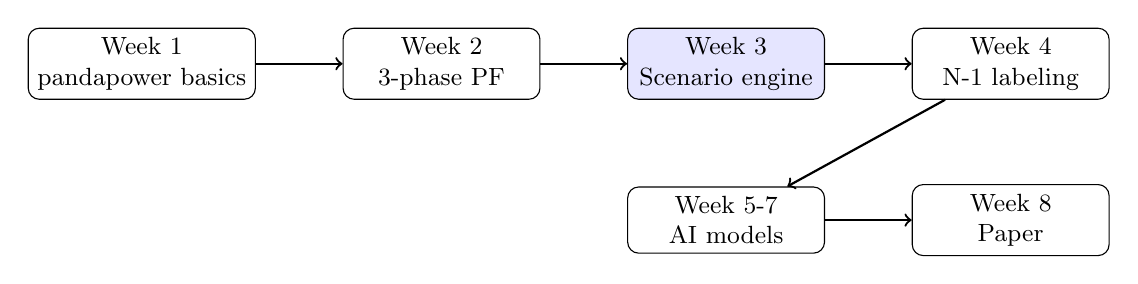
\begin{tikzpicture}[node distance=1.1cm, every node/.style={font=\small}]
\tikzstyle{box}=[draw, rounded corners, minimum width=2.5cm, minimum height=0.75cm, align=center]
\node[box] (w1) {Week 1\\pandapower basics};
\node[box, right=of w1] (w2) {Week 2\\3-phase PF};
\node[box, right=of w2, fill=blue!10] (w3) {Week 3\\Scenario engine};
\node[box, right=of w3] (w4) {Week 4\\N-1 labeling};
\node[box, below=of w3] (w5) {Week 5-7\\AI models};
\node[box, right=of w5] (w8) {Week 8\\Paper};
\draw[->, thick] (w1)--(w2);
\draw[->, thick] (w2)--(w3);
\draw[->, thick] (w3)--(w4);
\draw[->, thick] (w4)--(w5);
\draw[->, thick] (w5)--(w8);
\end{tikzpicture}
\vspace{0.5cm}

\textbf{Week 3 的产出：}一组经过验证的 base-case operating scenarios。\newline
\textbf{注意：}Week 3 不生成 N-1 labels；Week 4 才做 contingency scan。
\end{frame}

\begin{frame}{为什么 Week 3 很关键？}
\begin{block}{AI 安全预测的数据来源}
\[
\text{scenario } x_t + \text{contingency } c \longrightarrow \text{three-phase PF} \longrightarrow \text{violation label}
\]
\end{block}
\begin{itemize}
  \item 如果 scenario generator 有符号、reset 或设备配置错误，后续 N-1 labels 会被系统性污染。
  \item Week 3 的任务是保证 $x_t$ 本身物理合理、符号一致、可重复生成。
  \item Week 4 可以直接在每个 $x_t$ 上枚举 contingency $c$。
\end{itemize}
\end{frame}

\begin{frame}{Full feeder 与 teaching feeder}
\begin{columns}
\begin{column}{0.48\textwidth}
\textbf{Full feeder}\\
\begin{itemize}
  \item \texttt{ieee\_european\_lv\_asymmetric}
  \item 大型 LV asymmetric feeder proxy
  \item 适合后续研究实验与 benchmark
  \item 课堂初学阶段运行较慢，不利于逐步 debugging
\end{itemize}
\end{column}
\begin{column}{0.48\textwidth}
\textbf{Teaching feeder}\\
\begin{itemize}
  \item 9-bus radial microgrid-like feeder
  \item 0.4 kV, three-phase, asymmetric loads
  \item PV, BESS, EV, critical load 都可见
  \item 每个 proof 可手动审计
\end{itemize}
\end{column}
\end{columns}
\vspace{0.3cm}
\begin{block}{课程策略}
先用 teaching feeder 学会 pipeline，再迁移到 full feeder 或 reduced feeder。
\end{block}
\end{frame}

\begin{frame}{Microgrid story: 我们要模拟什么？}
\begin{columns}
\begin{column}{0.56\textwidth}
\begin{itemize}
  \item PCC: 上级电网连接点。
  \item Critical load: 重要负荷，后续可用于孤岛供电故事。
  \item PV: 单相或相别不均匀接入的 DER。
  \item BESS: 储能，Week 3 先作为静态充放电 setpoint。
  \item Operating scenario: 负荷、PV、BESS、相别不平衡的组合。
\end{itemize}
\end{column}
\begin{column}{0.42\textwidth}
\centering
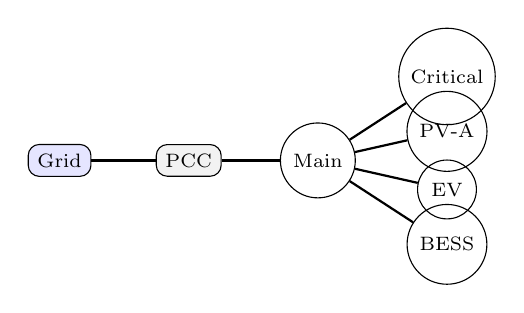
\begin{tikzpicture}[scale=0.82, every node/.style={font=\scriptsize}]
\node[draw, rounded corners, fill=blue!10] (grid) at (0,0) {Grid};
\node[draw, rounded corners, fill=gray!10] (pcc) at (2,0) {PCC};
\node[draw, circle] (main) at (4,0) {Main};
\node[draw, circle] (crit) at (6,1.3) {Critical};
\node[draw, circle] (pv) at (6,0.45) {PV-A};
\node[draw, circle] (ev) at (6,-0.45) {EV};
\node[draw, circle] (bess) at (6,-1.3) {BESS};
\draw[thick] (grid)--(pcc)--(main);
\draw[thick] (main)--(crit);
\draw[thick] (main)--(pv);
\draw[thick] (main)--(ev);
\draw[thick] (main)--(bess);
\end{tikzpicture}
\end{column}
\end{columns}
\end{frame}

\begin{frame}{Week 3 的数据流水线}
\centering
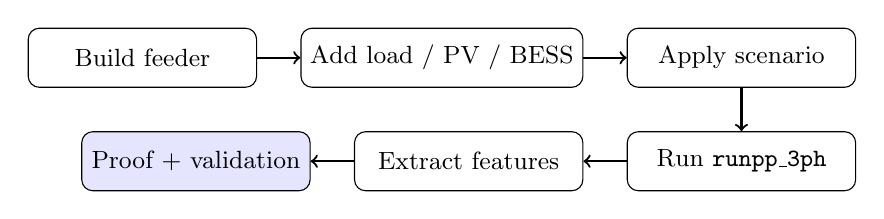
\begin{tikzpicture}[node distance=0.55cm, every node/.style={font=\small}]
\tikzstyle{box}=[draw, rounded corners, minimum width=2.9cm, minimum height=0.75cm, align=center]
\node[box] (load) {Build feeder};
\node[box, right=of load] (devices) {Add load / PV / BESS};
\node[box, right=of devices] (scen) {Apply scenario};
\node[box, below=of scen] (pf) {Run \texttt{runpp\_3ph}};
\node[box, left=of pf] (features) {Extract features};
\node[box, left=of features, fill=blue!10] (validate) {Proof + validation};
\draw[->, thick] (load)--(devices);
\draw[->, thick] (devices)--(scen);
\draw[->, thick] (scen)--(pf);
\draw[->, thick] (pf)--(features);
\draw[->, thick] (features)--(validate);
\end{tikzpicture}
\end{frame}

\begin{frame}{pandapower 三相元素回顾}
\begin{itemize}
  \item \texttt{runpp\_3ph()} 用于 asymmetric / three-phase power flow。
  \item \texttt{asymmetric\_load}: A/B/C 三相负荷，load convention 下正有功表示消耗。
  \item \texttt{asymmetric\_sgen}: A/B/C 三相静态发电，generator convention 下正有功表示注入。
  \item 三相线路需要正序和零序参数，用于 sequence-frame 三相潮流。
\end{itemize}
\begin{block}{Week 3 使用原则}
PV 用 \texttt{asymmetric\_sgen}；BESS 放电用 \texttt{asymmetric\_sgen}；BESS 充电用 \texttt{asymmetric\_load}。
\end{block}
\end{frame}

\begin{frame}{Teaching feeder 的组成}
\begin{table}
\centering
\scriptsize
\begin{tabular}{ll}
\toprule
Component & Purpose \\
\midrule
PCC bus + ext grid & grid-connected mode slack equivalent \\
Main bus & feeder root after PCC \\
Critical load bus & high-priority load \\
Residential bus & ordinary load \\
EV bus & high-demand flexible load \\
Remote bus & voltage-sensitive feeder end \\
Medical bus & another critical load example \\
PV-A / PV-C buses & single-phase DER injections \\
BESS-like pair & charge/discharge static setpoint \\
\bottomrule
\end{tabular}
\end{table}
\end{frame}

\begin{frame}[fragile]{代码结构: feeder builder}
\begin{lstlisting}[language=Python]
def create_microgrid_teaching_feeder():
    net = pp.create_empty_network(...)
    create buses
    create ext_grid at PCC
    create lines with sequence parameters
    create asymmetric_load elements
    create asymmetric_sgen PV placeholders
    create BESS charge load and discharge sgen
    return net, metadata
\end{lstlisting}
\begin{block}{metadata 的作用}
保存 bus map、line names、original load indices、PV config 和 BESS config，便于 scenario apply 与 validation。
\end{block}
\end{frame}

\begin{frame}{Proof 1: 输入网络完整性}
\begin{itemize}
  \item 必要表存在：bus, line, ext\_grid, asymmetric\_load, asymmetric\_sgen。
  \item 所有 element 的 bus 引用必须合法。
  \item line zero-sequence columns 必须存在。
  \item 网络从 PCC 看必须 connected。
  \item teaching feeder 设计为 radial，方便学生理解潮流方向与设备影响。
\end{itemize}
\begin{block}{为什么这一步重要？}
如果网络结构都不可信，后面所有 scenario 和 AI label 都没有意义。
\end{block}
\end{frame}

\begin{frame}{Scenario table: 参数定义}
\begin{table}
\centering
\scriptsize
\begin{tabular}{ll}
\toprule
Parameter & Meaning \\
\midrule
\texttt{load\_scale} & 全局负荷缩放 \\
\texttt{phase\_a/b/c\_factor} & A/B/C 相额外缩放，用于制造相别不平衡 \\
\texttt{pv\_scale} & PV 出力缩放 \\
\texttt{bess\_p\_discharge\_mw} & BESS 净放电功率，正为放电，负为充电 \\
\texttt{mode} & Week 3 固定为 grid\_connected \\
\bottomrule
\end{tabular}
\end{table}
\end{frame}

\begin{frame}{Deterministic scenarios}
\begin{table}
\centering
\scriptsize
\begin{tabular}{lrrrrl}
\toprule
Scenario & Load & A & B & C & Purpose \\
\midrule
base & 1.00 & 1.00 & 1.00 & 1.00 & reference \\
high\_load & 1.25 & 1.00 & 1.00 & 1.00 & voltage/loading stress \\
high\_pv\_midday & 0.75 & 1.00 & 1.00 & 1.00 & high DER injection \\
phase\_b\_heavy & 1.00 & 1.00 & 1.60 & 1.00 & VUF stress \\
evening\_peak & 1.35 & 1.00 & 1.00 & 1.00 & BESS discharge \\
stress\_unbalance & 1.45 & 0.75 & 1.80 & 0.90 & difficult case \\
\bottomrule
\end{tabular}
\end{table}
\end{frame}

\begin{frame}[fragile]{Random scenarios}
\begin{itemize}
  \item Deterministic scenarios 用于教学和 debugging。
  \item Random scenarios 用于后续扩大 AI dataset。
  \item 必须固定 random seed，确保实验可复现。
\end{itemize}
\begin{lstlisting}[language=Python]
rng = np.random.default_rng(seed)
load_scale = rng.uniform(0.70, 1.60)
phase_factors = clip(Normal(1.0, 0.18), 0.65, 1.55)
pv_scale = rng.uniform(0.0, 1.4)
bess_setpoint = rng.uniform(-0.012, 0.012)
\end{lstlisting}
\end{frame}

\begin{frame}[fragile]{Scenario apply 的核心原则}
\begin{block}{Reset before apply}
每次应用新场景前，都必须恢复原始 load 和 sgen 输入表。
\end{block}
\begin{lstlisting}[language=Python]
def reset_input_state(net, base_load, base_sgen):
    net.asymmetric_load.loc[:, cols] = base_load.loc[:, cols]
    net.asymmetric_sgen.loc[:, cols] = base_sgen.loc[:, cols]

apply_scenario(...):
    reset_input_state(...)
    apply_load_scaling(...)
    apply_pv_setpoints(...)
    apply_bess_setpoint(...)
\end{lstlisting}
\end{frame}

\begin{frame}{Proof 2: idempotence check}
\begin{block}{定义}
对同一个 scenario 连续应用两次，输入表签名必须完全一致。
\end{block}
\[
\mathrm{signature}(A(A(x,s),s)) = \mathrm{signature}(A(x,s))
\]
\begin{itemize}
  \item 这里 $A$ 表示 apply scenario 操作。
  \item signature 包括 load/sgen 的各相 P/Q 总和和绝对值总和。
  \item 如果检查失败，通常说明没有 reset 或某个 multiplier 被累积。
\end{itemize}
\end{frame}

\begin{frame}{BESS setpoint mapping}
\begin{columns}
\begin{column}{0.48\textwidth}
\textbf{Discharge}\
\[
P_{BESS}>0
\]
\begin{itemize}
  \item 写入 \texttt{asymmetric\_sgen}
  \item 代表向网络注入有功
  \item PCC import 应下降
\end{itemize}
\end{column}
\begin{column}{0.48\textwidth}
\textbf{Charge}\
\[
P_{BESS}<0
\]
\begin{itemize}
  \item 写入 \texttt{asymmetric\_load}
  \item 代表从网络消耗有功
  \item PCC import 应上升
\end{itemize}
\end{column}
\end{columns}
\end{frame}

\begin{frame}{Proof 3: BESS sign convention}
\begin{itemize}
  \item 构造三个仅 BESS setpoint 不同的测试 case：base、charge、discharge。
  \item 检查 BESS 放电时 \texttt{asymmetric\_sgen} 增加。
  \item 检查 BESS 充电时 \texttt{asymmetric\_load} 增加。
  \item 检查三相潮流结果：
\end{itemize}
\[
P^{grid}_{charge} > P^{grid}_{base} > P^{grid}_{discharge}
\]
\end{frame}

\begin{frame}[fragile]{三相潮流运行}
\begin{lstlisting}[language=Python]
pp.runpp_3ph(
    net,
    calculate_voltage_angles=True,
    init="auto",
    max_iteration=60,
    tolerance_mva=1e-7,
)
\end{lstlisting}
\begin{itemize}
  \item 提取 \texttt{res\_bus\_3ph}: 三相电压、角度、VUF。
  \item 提取 \texttt{res\_line\_3ph}: 三相电流、loading、loss。
  \item 提取 \texttt{res\_ext\_grid\_3ph}: PCC 三相 P/Q。
\end{itemize}
\end{frame}

\begin{frame}{Base-case security summary}
\begin{table}
\centering
\scriptsize
\begin{tabular}{ll}
\toprule
Feature & Meaning \\
\midrule
\texttt{min\_vm\_pu} & 所有 bus-phase 中最低相电压 \\
\texttt{max\_vm\_pu} & 所有 bus-phase 中最高相电压 \\
\texttt{max\_vuf\_percent} & 最大 voltage unbalance factor \\
\texttt{max\_line\_loading\_percent} & 最大相线路 loading \\
\texttt{p\_grid\_mw}, \texttt{q\_grid\_mvar} & PCC 有功/无功交换 \\
\texttt{p\_load\_a/b/c\_mw} & 三相负荷总量 \\
\texttt{p\_sgen\_a/b/c\_mw} & 三相 DER/BESS 注入 \\
\bottomrule
\end{tabular}
\end{table}
\end{frame}

\begin{frame}{Proof 4: active-power accounting}
对每个场景检查：
\[
P_{grid}+P_{sgen}-P_{load}-P_{line\ loss}\approx 0
\]
\begin{itemize}
  \item 这个检查不会替代潮流算法本身。
  \item 它用于验证结果表之间的物理账本是否一致。
  \item 如果 residual 很大，常见原因是符号约定错、结果表没更新、或漏掉某类设备。
\end{itemize}
\end{frame}

\begin{frame}{Proof 5: manual VUF calculation}
对每个 bus，从结果表重建相量：
\[
V_a,\quad V_b,\quad V_c
\]
用对称分量计算：
\[
V_1 = \frac{V_a + \alpha V_b + \alpha^2 V_c}{3},\quad
V_2 = \frac{V_a + \alpha^2 V_b + \alpha V_c}{3}
\]
\[
\mathrm{VUF}=100\frac{|V_2|}{|V_1|}
\]
然后与 \texttt{res\_bus\_3ph.unbalance\_percent} 比较。
\end{frame}

\begin{frame}{Proof 6: manual line loading check}
对每条 line，使用结果表中的相电流和线路额定电流复核：
\[
\mathrm{loading}_{\ell,\phi} = 100\frac{I_{\ell,\phi}}{I^{max}_{\ell}}
\]
\begin{itemize}
  \item 手算 loading 与 pandapower 结果表比较。
  \item 检查每相 loading，也检查 total \texttt{loading\_percent}。
  \item 这一步帮助学生理解 loading 不是黑箱变量。
\end{itemize}
\end{frame}

\begin{frame}[fragile]{Proof 7: cross-copy reproducibility}
\begin{lstlisting}[language=Python]
net1 = create_microgrid_teaching_feeder()
net2 = create_microgrid_teaching_feeder()

run_scenario(net1, scenario)
run_scenario(net2, scenario)

assert max_abs_difference < tolerance
\end{lstlisting}
\begin{itemize}
  \item 从零构建两个独立网络副本。
  \item 对同一个 scenario 运行三相潮流。
  \item 比较电压、VUF、loading、电流和 grid import。
\end{itemize}
\end{frame}

\begin{frame}{Proof 8: engineering trend checks}
\begin{itemize}
  \item high load: 总负荷应增加，最低电压通常下降，线路 loading 上升。
  \item high PV: DER 注入增加，PCC grid import 应下降。
  \item phase-B-heavy: 最大 VUF 应高于 base。
  \item stress scenario: VUF 或 loading 至少应比 base 更严重。
  \item BESS charge/discharge: 充电增加 grid import，放电降低 grid import。
\end{itemize}
\begin{block}{定位}
这些不是数学定理，而是工程 sanity checks，用来快速发现符号和场景应用错误。
\end{block}
\end{frame}

\begin{frame}{Validation summary}
Notebook 会输出 \texttt{week3\_validation\_test\_summary.csv}，包含：
\begin{itemize}
  \item input network integrity
  \item scenario table schema
  \item scenario application idempotence
  \item BESS sign convention
  \item active power balance
  \item manual VUF check
  \item manual line loading check
  \item copy reproducibility
  \item repeated run reproducibility
  \item engineering trend checks
  \item AI feature schema
\end{itemize}
\end{frame}

\begin{frame}{从 Week 3 到 Week 4}
Week 3 生成：
\[
\mathcal{X}=\{x_1,x_2,\ldots,x_T\}
\]
每个 $x_t$ 是一个 base-case operating scenario。

Week 4 将加入 contingency set：
\[
\mathcal{C}=\{c_1,c_2,\ldots,c_K\}
\]
生成：
\[
(x_t,c_k) \rightarrow y_{t,k},\quad s_{t,k}
\]
\begin{block}{Week 4 的标签}
phase voltage violation, phase current violation, VUF violation, non-convergence。
\end{block}
\end{frame}

\begin{frame}{Week 3 输出文件}
\begin{table}
\centering
\scriptsize
\begin{tabular}{ll}
\toprule
File & Purpose \\
\midrule
\texttt{week3\_scenario\_table.csv} & 场景定义表 \\
\texttt{week3\_pv\_config.csv} & PV bus、相别、容量配置 \\
\texttt{week3\_bess\_config.csv} & BESS charge/discharge 配置 \\
\texttt{week3\_scenario\_security\_summary.csv} & 每个场景的 base-case 安全摘要 \\
\texttt{week3\_basecase\_ai\_features.csv} & Week 4/5 使用的基础特征表 \\
\texttt{week3\_validation\_test\_summary.csv} & 所有 proof / validation 结果 \\
\bottomrule
\end{tabular}
\end{table}
\end{frame}

\begin{frame}{学生课堂任务}
\begin{enumerate}
  \item 运行 clean notebook，确认所有 validation tests 通过。
  \item 解释 high load、high PV、phase-B-heavy 三个场景的物理意义。
  \item 查看 \texttt{week3\_scenario\_security\_summary.csv}，找出最低电压场景。
  \item 查看 \texttt{max\_vuf\_percent}，找出最不平衡场景。
  \item 修改一个场景参数，并判断结果趋势是否合理。
\end{enumerate}
\end{frame}

\begin{frame}{课后练习}
\begin{enumerate}
  \item 新增 \texttt{phase\_c\_heavy} 场景，与 \texttt{phase\_b\_heavy} 比较 VUF。
  \item 新增 \texttt{low\_load\_high\_pv} 场景，观察 \texttt{max\_vm\_pu} 是否上升。
  \item 生成 50 个 random scenarios，并按 \texttt{max\_vuf\_percent} 排序。
  \item 新增 base-case risk flag: \(\mathbb{I}(\min V <0.95 \text{ or } \max loading>100\%)\)。
  \item 写一段话说明 Week 3 的 features 如何扩展为 Week 4 的 N-1 labels。
\end{enumerate}
\end{frame}

\begin{frame}{常见错误与排查}
\begin{table}
\centering
\scriptsize
\begin{tabular}{p{0.35\textwidth}p{0.54\textwidth}}
\toprule
错误 & 排查方法 \\
\midrule
场景结果越来越极端 & 检查是否每次 scenario 前 reset base input \\
PV 后 grid import 增加 & 检查 sgen 和 load 的符号约定 \\
BESS 充放电趋势相反 & 检查 \texttt{bess\_p\_discharge\_mw} 映射 \\
VUF 没有变化 & 检查 phase factor 是否作用到 A/B/C 负荷列 \\
结果表缺列 & 检查 \texttt{runpp\_3ph()} 是否成功和 pandapower 版本 \\
\bottomrule
\end{tabular}
\end{table}
\end{frame}

\begin{frame}{论文写作中的 Week 3 价值}
\begin{itemize}
  \item 在论文中，Week 3 对应 \textbf{Dataset generation and scenario design}。
  \item 它说明训练数据不是任意拼接，而是来自物理建模与可复现实验流程。
  \item proof / validation 可以写成 reproducibility 和 data-quality control。
  \item 它为后面 N-1 label、AI baseline、physics-informed loss 提供可信数据基础。
\end{itemize}
\begin{block}{建议论文表述}
We first construct a three-phase microgrid scenario generation pipeline and validate each operating point using power-flow convergence, power-balance residuals, sign-convention checks, and engineering trend tests.
\end{block}
\end{frame}

\begin{frame}{小结}
\begin{itemize}
  \item Week 3 把三相潮流从单个 case 扩展为可复现的 scenario engine。
  \item teaching feeder 让学生能在课堂中快速运行和手动验证。
  \item 我们定义了 deterministic 和 random 两类 scenario。
  \item 我们提取了 Week 4/5 需要的 base-case AI features。
  \item 最重要的是：用 proof 和 cross-validation 检查符号、重置、物理平衡、趋势和复现性。
\end{itemize}
\end{frame}

\begin{frame}{参考资料}
\scriptsize
\begin{itemize}
  \item pandapower documentation: \texttt{runpp\_3ph}, asymmetric three-phase power flow.
  \item pandapower documentation: \texttt{ieee\_european\_lv\_asymmetric}, 3-phase grid data.
  \item pandapower documentation: \texttt{asymmetric\_load}, \texttt{asymmetric\_sgen}, and unit conventions.
\end{itemize}
\vspace{0.4cm}
本课程后续 Week 4 将基于本周输出文件进行三相 N-1 contingency labeling。
\end{frame}

\end{document}
